\chapter{Robot minisumo}

W niniejszym rozdziale opisany został proces tworzenia robota minisumo. Wyróżniono w nim trzy główne sekcje: \textit{Konstrukcja}, \textit{Elektronika} oraz \textit{Oprogramowanie}.

\begin{figure}[H]
	\centering
		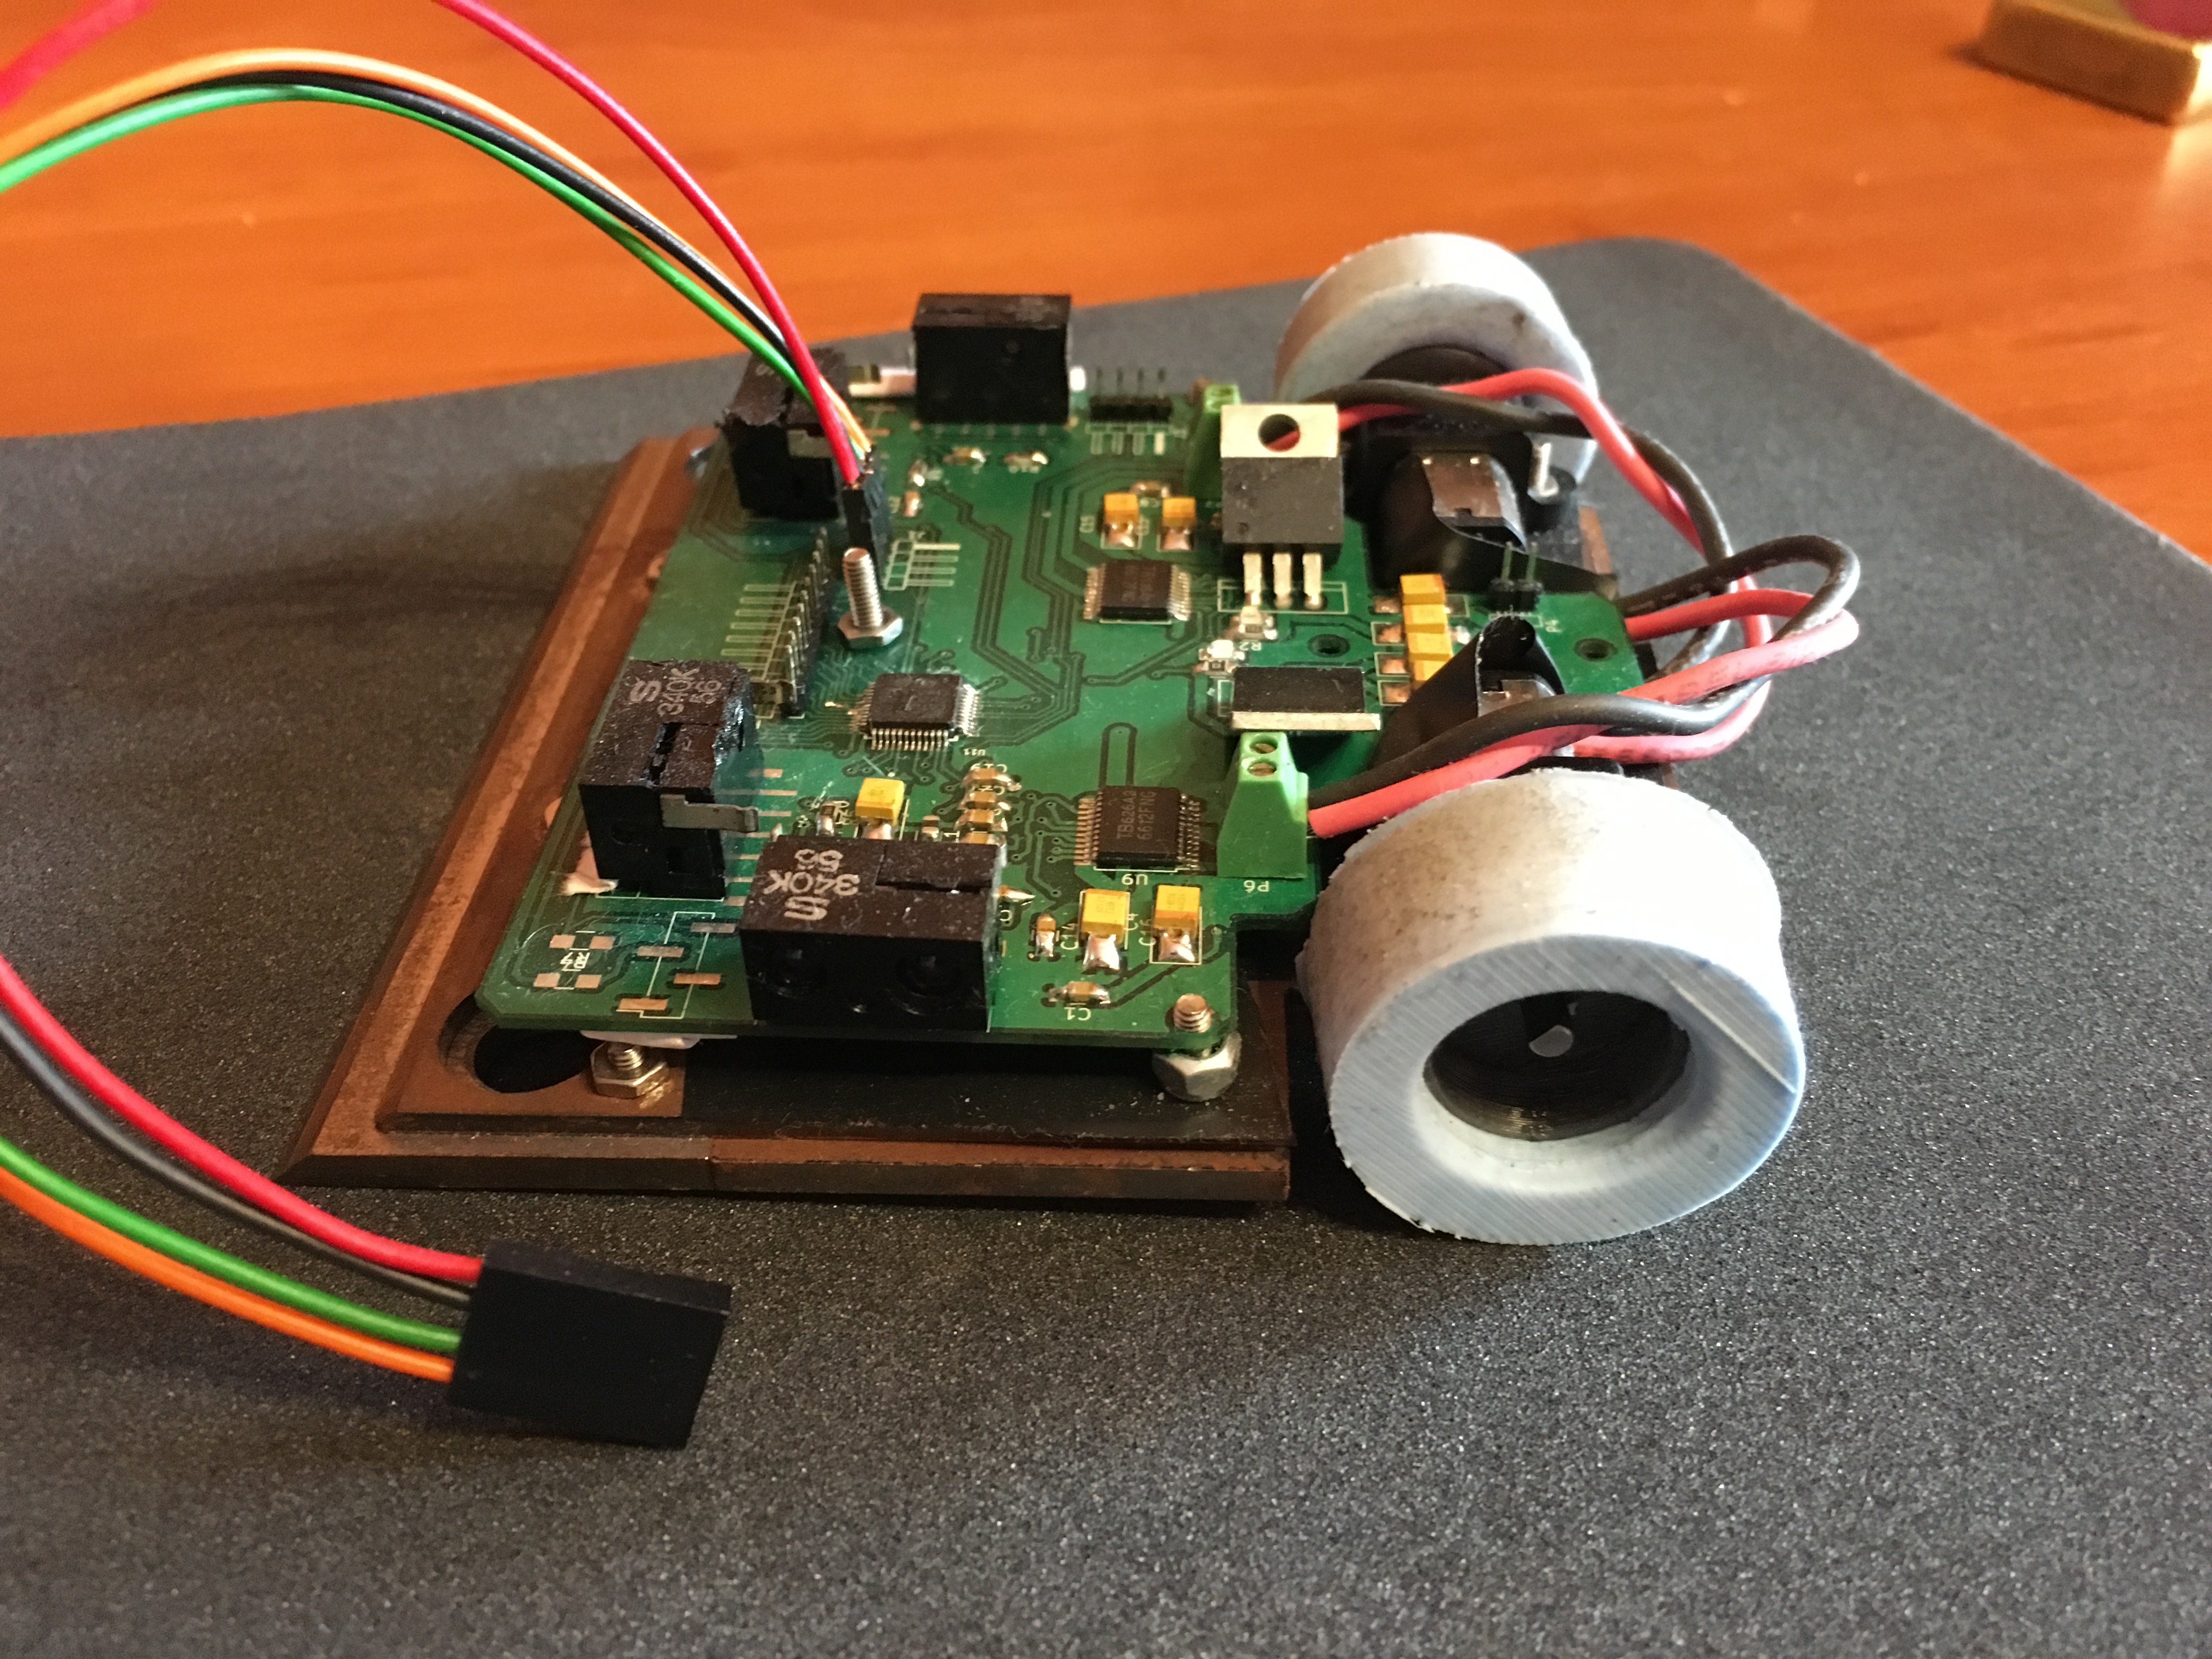
\includegraphics[width=0.75\linewidth]{pic04/minisumo.JPG}
	\caption{Wykonany robot minisumo.}
	\label{fig:robot}	
\end{figure}

Zdjęcie ~\ref{fig:robot} przedstawia omawianego robota minisumo. W celu ukazania elektroniki ściągnięto nadwozie.

\section{Konstrukcja}
\subsection{Założenia}
Głównym założeniem konstrukcyjnym było zminimalizowanie szansy podbicia robota przez przeciwnika. W związku z czym napęd robota składa się z dwóch kół umiejscowionych w tylnej części konstrukcji. Przednia część robota zakończona jest pługiem, który bezpośrednio dotyka podłoża. Dodatkowo starano się, aby środek ciężkości całej konstrukcji znajdował się jak najbliżej podłoża.

\subsection{Nadwozie}
Konstrukcja nadwozia została zaprojektowana przy użyciu środowiska \textit{Autodesk Inventor 2017}. Wybór został podyktowany łatwością obsługi narzędzi oraz darmową licencją studencką. Obudowa została wykonana w technologii druku 3D, ze względu na małą masę, koszt produkcji oraz możliwość łatwego dostosowania do potrzeb projektu (otwory na śruby oraz czujniki przeciwnika, przestrzeń na koła).  

\begin{figure}[H]
	\centering
		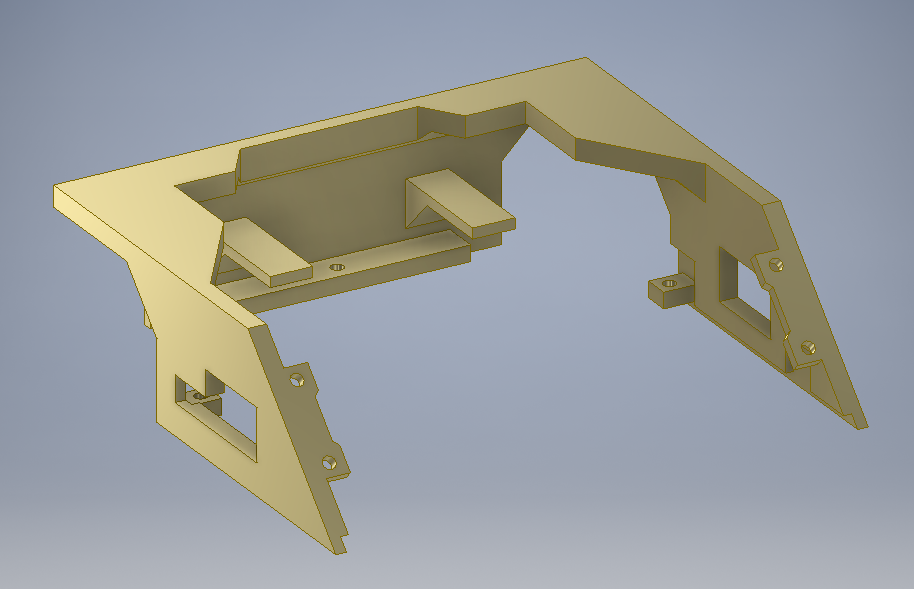
\includegraphics[width=0.75\linewidth]{pic04/body.png}
	\caption{Projekt nadwozia w środowisku Autodesk Inventor 2017.}
	\label{fig:body}	
\end{figure}

Na ilustracji ~\ref{fig:body} znajduje się projekt nadwozia robota. Ze względu na niewielką wytrzymałość plastikowego wydruku przywiązano dużą wagę do szerokości obudowy. Starano się, aby była możliwie jak najszersza, co skutkowało wzrostem trwałości całej konstrukcji. Dodatkowo front robota został wykonany ze stali, ponieważ w przypadku podważenia przeciwnika jest obszarem najbardziej podatnym na zniszczenia. 

\subsection{Podwozie}
Całość podwozia wykonana została ze stali ze względu na wytrzymałość oraz dużą masę, która przyczyniła się do znacznego obniżenia środka ciężkości konstrukcji.  Podobnie jak w przypadku nadwozia projekt został stworzony w środowisku \textit{Autodesk Inventor 2017}. Konstrukcja składa się z trzech płytek, z czego jedna zawiera ostrze od strugarki, wykonane z węglika spiekanego. Materiał ten cechuje się wysoką wytrzymałością oraz większą odpornością na kruszenie w porównaniu do zwykłej stali. 

\begin{figure}[H]
	\centering
		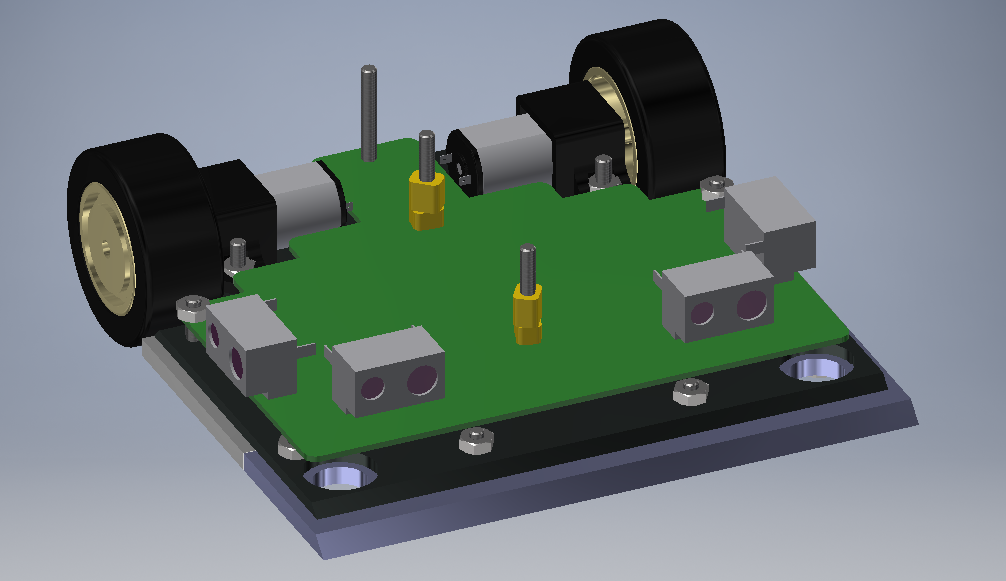
\includegraphics[width=0.75\linewidth]{pic04/chassis.png}
	\caption{Projekt podwozia w środowisku Autodesk Inventor 2017.}
	\label{fig:chassis}	
\end{figure}

Ilustracja ~\ref{fig:chassis} ukazuje wizualizację podwozia wraz z silnikami oraz kołami. Projekt wyeksportowano do formatu 2D, a następnie wykonano przy użyciu techniki wypalania laserem. 

\subsection{Napęd}
Jak wspomniano wcześniej, napęd robota składa się z dwóch kół, które sterowane są niezależnie. Ruch robota wzorowany jest na zasadzie działania czołgu. W przypadku skrętu, do jednego z silników dostarczana jest większa moc, co skutkuje wzrostem prędkości kątowej napędzanego koła. Z powodu różnicy prędkości kół robot zaczyna skręcać. Zdecydowano się na takie rozwiązanie ze względu na dozwoloną masę (większa ilość kół oraz silników znacząco by ją zwiększyła) oraz manewrowość – dzięki zastosowaniu omawianego rozwiązania możliwy jest obrót robota w miejscu (w przypadku, gdy koła kręcą się w przeciwne strony), dzięki czemu pojazd jest szybki oraz zwinny. 

\begin{figure}[H]
	\centering
		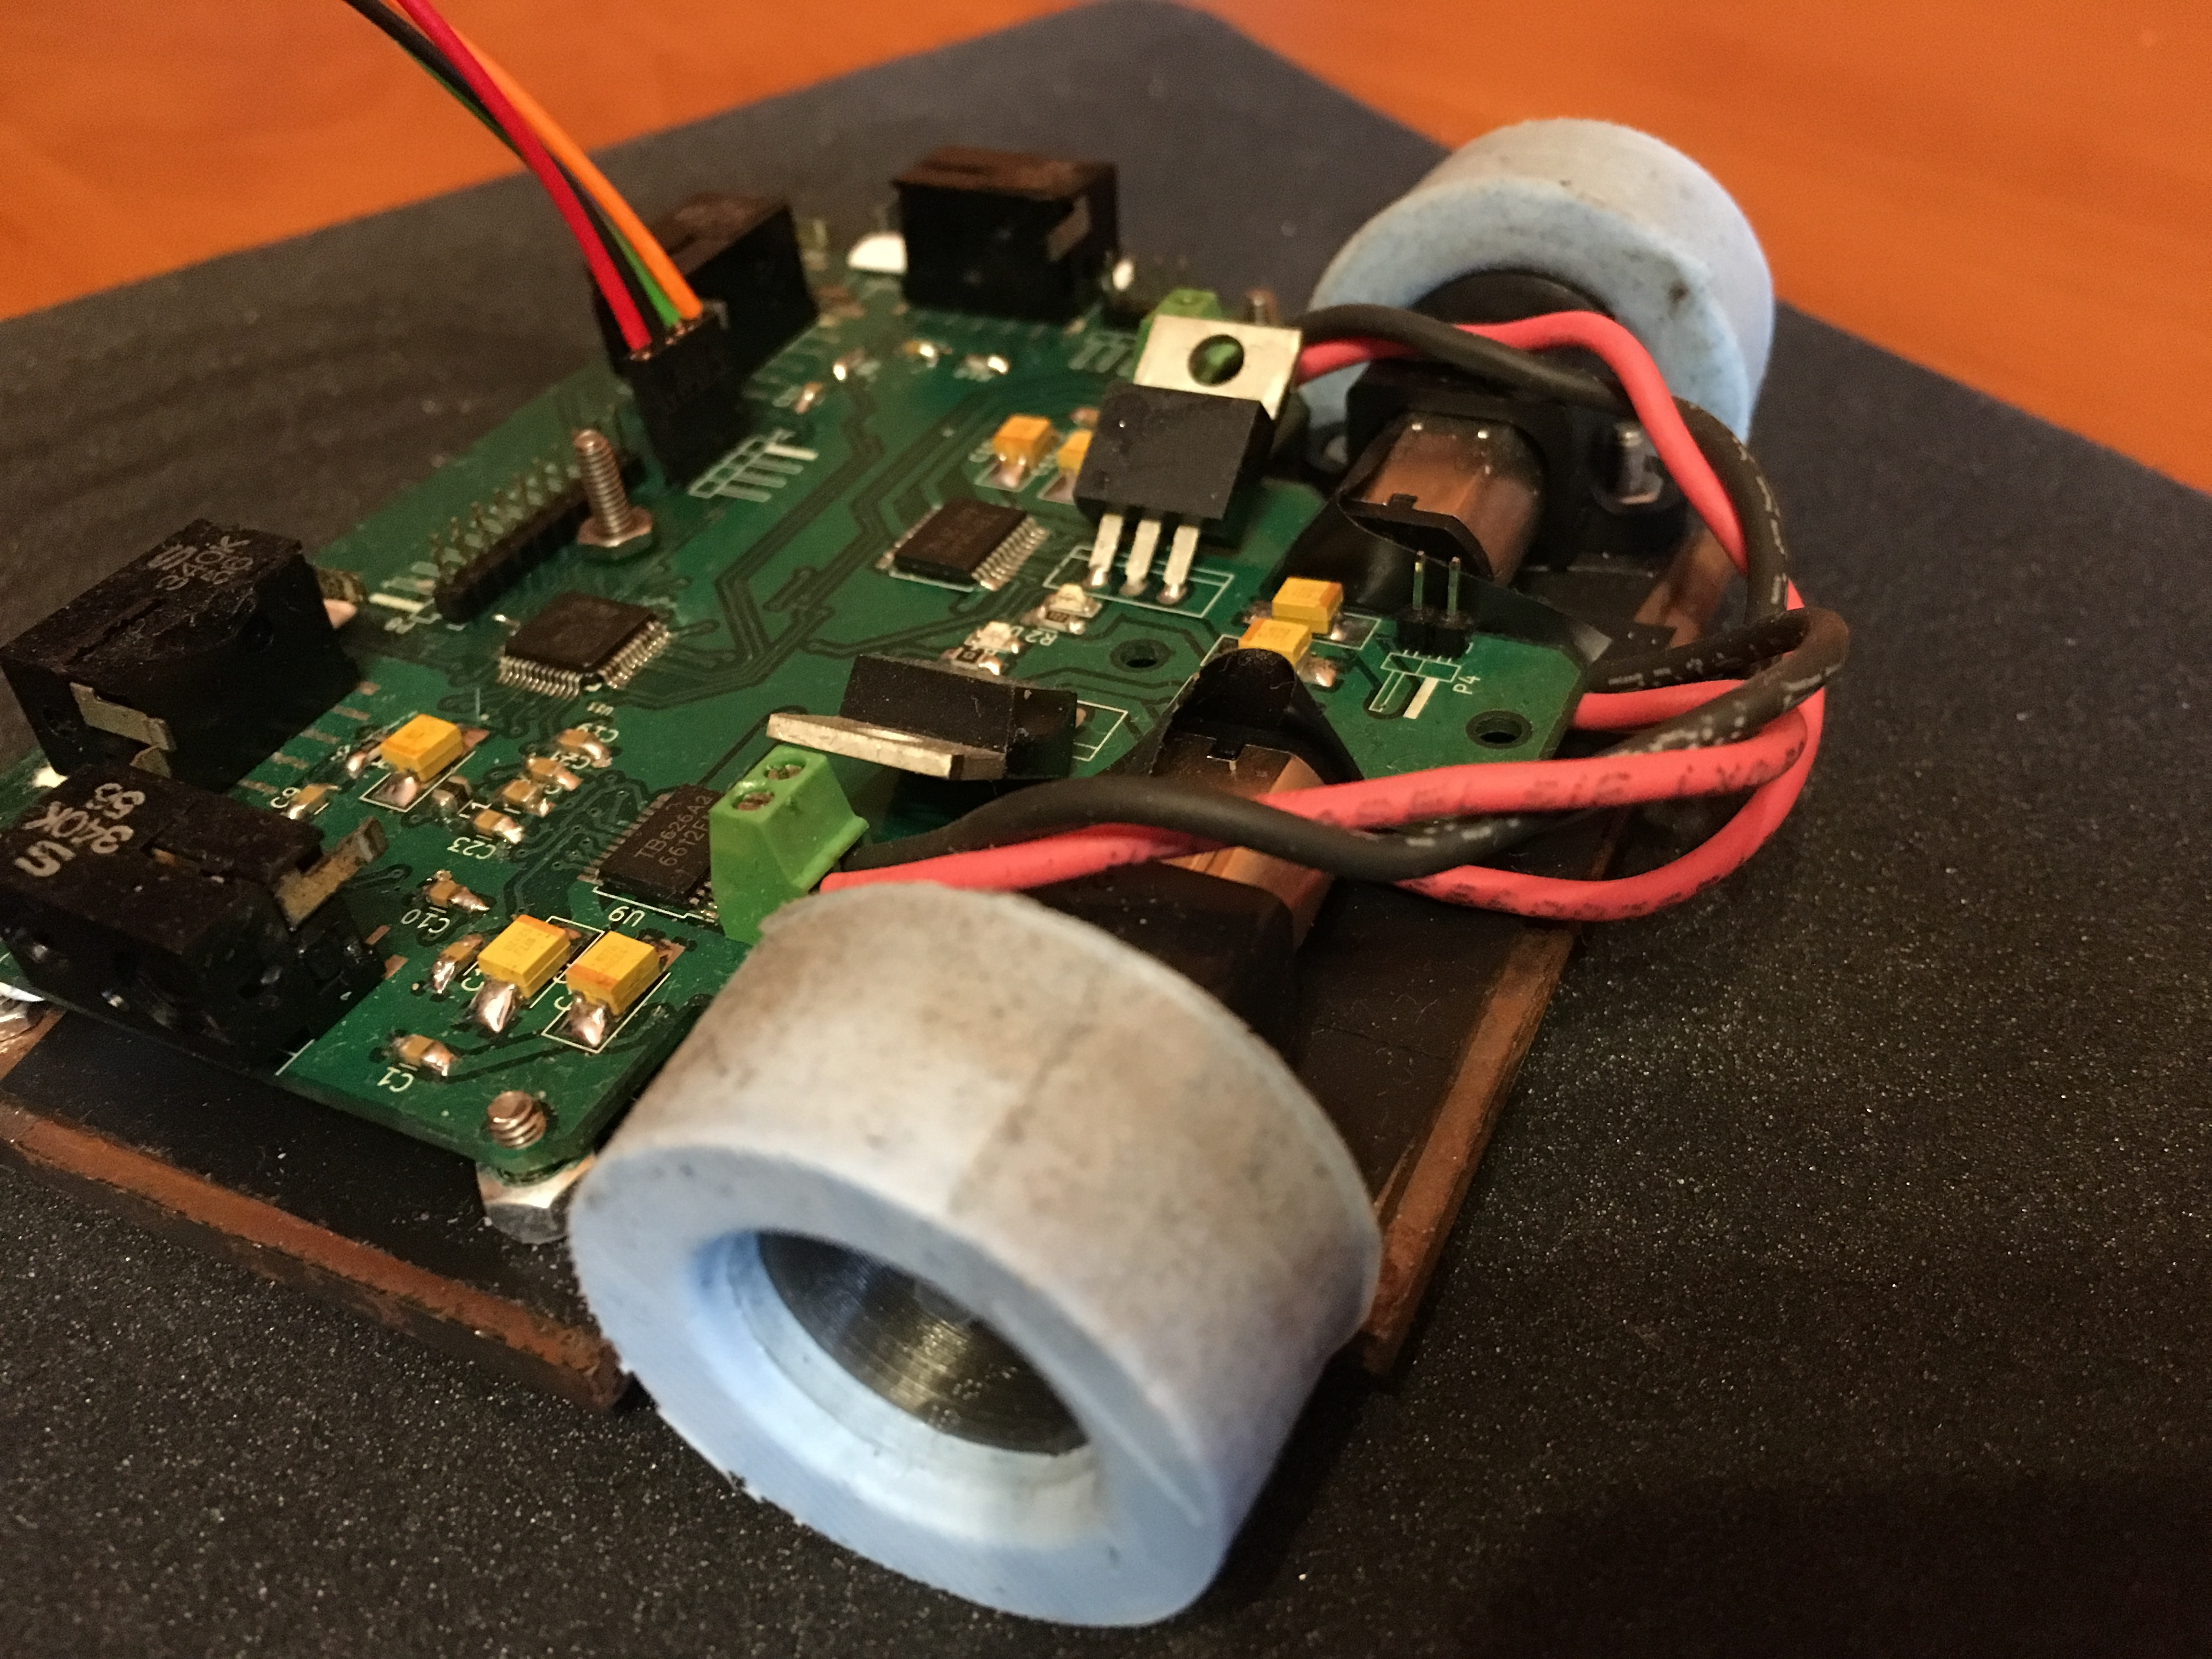
\includegraphics[width=0.75\linewidth]{pic04/drive.JPG}
	\caption{Napęd robota minisumo.}
	\label{fig:drive}	
\end{figure}

Na zdjęciu ~\ref{fig:drive} przedstawiono napęd robota na który składają się dwa silniki oraz dwie felgi z oponami. Jako jednostkę napędową użyto silników \textit{Pololu HPCB} ze względu  na rozmiary, dopuszczalne napięcie zasilania oraz korzystny stosunek ceny do jakości. Felgi zostały wykonane przy pomocy wydruku 3D, a opony były gotowym komponentem wykonanym z poliuretanu.

\section{Elektronika}
Projekt elektroniki robota, będącego tematem pracy dyplomowej, został stworzony przy użyciu darmowego środowiska \textit{KiCad}. Z początku płytki zostały wykonane własnoręcznie za pomocą metody termotransferu. Aczkolwiek z powodu dużej ilości przelotek, braku odpowiednich narzędzi oraz kilku błędów popełnionych na etapie projektowania, stwierdzono, iż lepszym rozwiązaniem będzie przeprojektowanie płytki oraz zlecenie wydruku firmie specjalizującej się w~tej dziedzinie. Nowa płytka była zdecydowanie trwalsza od poprzedniej wersji. Ponadto dzięki zastosowaniu soldermaski oraz cynowania HAL lutowanie elementów okazało się znacznie łatwiejsze.  

Docelowo robot posiada dwie płytki:
\begin{itemize}
\item główną – zawierającą całą logikę robota,
\item interfejs – pełniący rolę interfejsu użytkownika, posiadający przyciski oraz diody LED.
\end{itemize}


\begin{figure}[H]
	\centering
		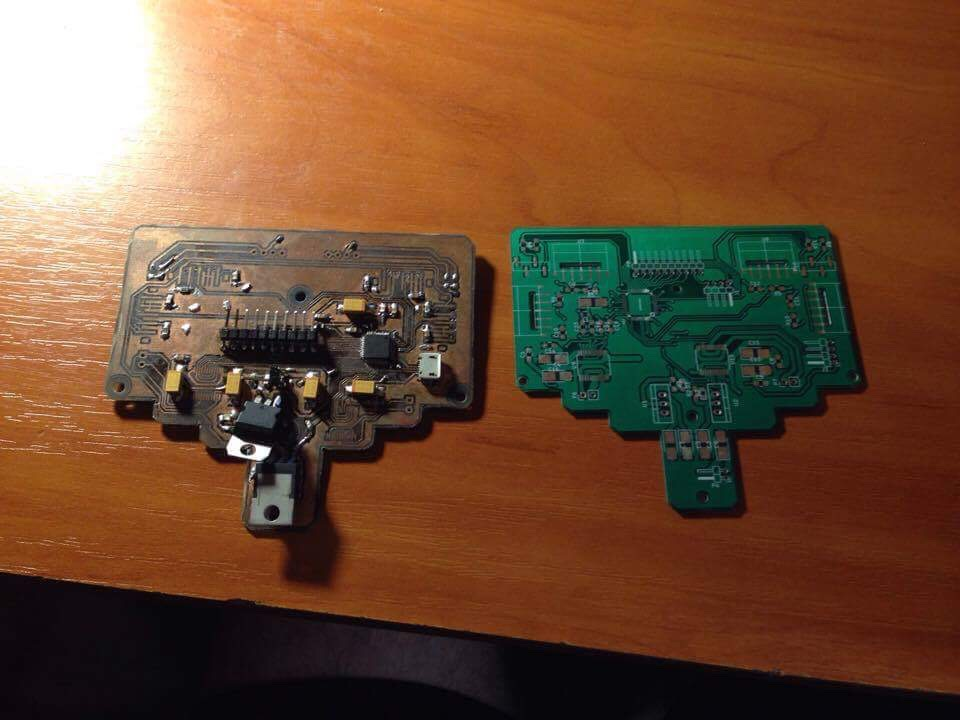
\includegraphics[width=0.75\linewidth]{pic04/boards.JPG}
	\caption{Porównanie wykonanych płytek drukowanych.}
	\label{fig:boards}	
\end{figure}

Na zdjęciu ~\ref{fig:boards} przedstawiono pierwszą  (wykonaną metodą termotransferu) oraz finalną (wykonaną przez firmę) wersję górnej płytki.  

\subsection{Układ zasilania}
Ze względu na ograniczone miejsce oraz dozwoloną masę za źródło zasilania posłużył akumulator litowo–polimerowy (Li–Pol) posiadający dwie cele oraz 400mAh pojemności. Bateria cechowała się wystarczającą wydajnością prądową, a pojemność pozwalała na stoczenie kilku pojedynków bez potrzeby ładowania. 

Z racji iż nie wszystkie elementy elektroniki tolerują napięcie 7.4V, układ zasilania został wyposażony w stabilizatory 3.3V oraz 5V. 

\subsection{Procesor}
Poniżej wymieniono niezbędne funkcjonalności jakie musiała spełniać docelowa jednostka obliczeniowa:

\begin{itemize}
\item przetwornik analogowo – cyfrowy (\textit{ang. ADC – analog to digital converter)} potrzebny do obsługi czujników końca ringu,
\item odpowiednia ilość portów wejścia/wyjścia dla przycisków oraz diod,
\item możliwość zmiany wypełnienia sygnału prądowego lub napięciowego (\textit{ang. PWM – Pulse–Width Modulation}) w celu odpowiedniego sterowania mocą silników,
\item interfejs UART (\textit{ang. Universal Synchronous and Asynchronous Reciever and Transmitter}) niezbędny przy komunikacji z modułem Bluetooth,
\item obsługa przerwań wykorzystywana w odbiorze wiadomości.
\end{itemize}

Powyższe wymagania spełniał procesor \textit{STM32F100C8T6B - LQFP48}. Dodatkowymi atutami była niska cena, ogólnodostępność oraz małe rozmiary.

\subsection{Sensoryka}
Konstrukcja została wyposażona w cztery czujniki \textit{SHARP Gp2y0d340k} wykrywające obecność przeciwnika do 40 centymetrów. Umieszczono je z przodu robota – dwa po bokach oraz dwa od frontu. Dodatkowo przy pługu znajdują się dwa czujniki sygnalizujące opuszczenie pola walki.

\subsection{Sterownik silników}
Jako sterownik posłużył dwukanałowy, 1.2 amperowy mostek H \textit{TB6612}. Wybór został podyktowany dostępnością oraz ceną. Aczkolwiek z czasem okazało się, iż omawiany układ jest bardzo awaryjny, szczególnie nie nadaje się do walki w zwarciu.

\subsection{Schemat elektroniki}
W celu zwiększenia czytelności schemat podzielono na moduły, które podpisano oraz obramowano niebieską linią. 

Poniżej na zdjęciu ~\ref{fig:electric_scheme} przedstawiono schemat zaprojektowanej elektroniki (zarówno płytki górnej, jak i interfejsu).
\begin{landscape}
\begin{figure}[ht]
	\centering
		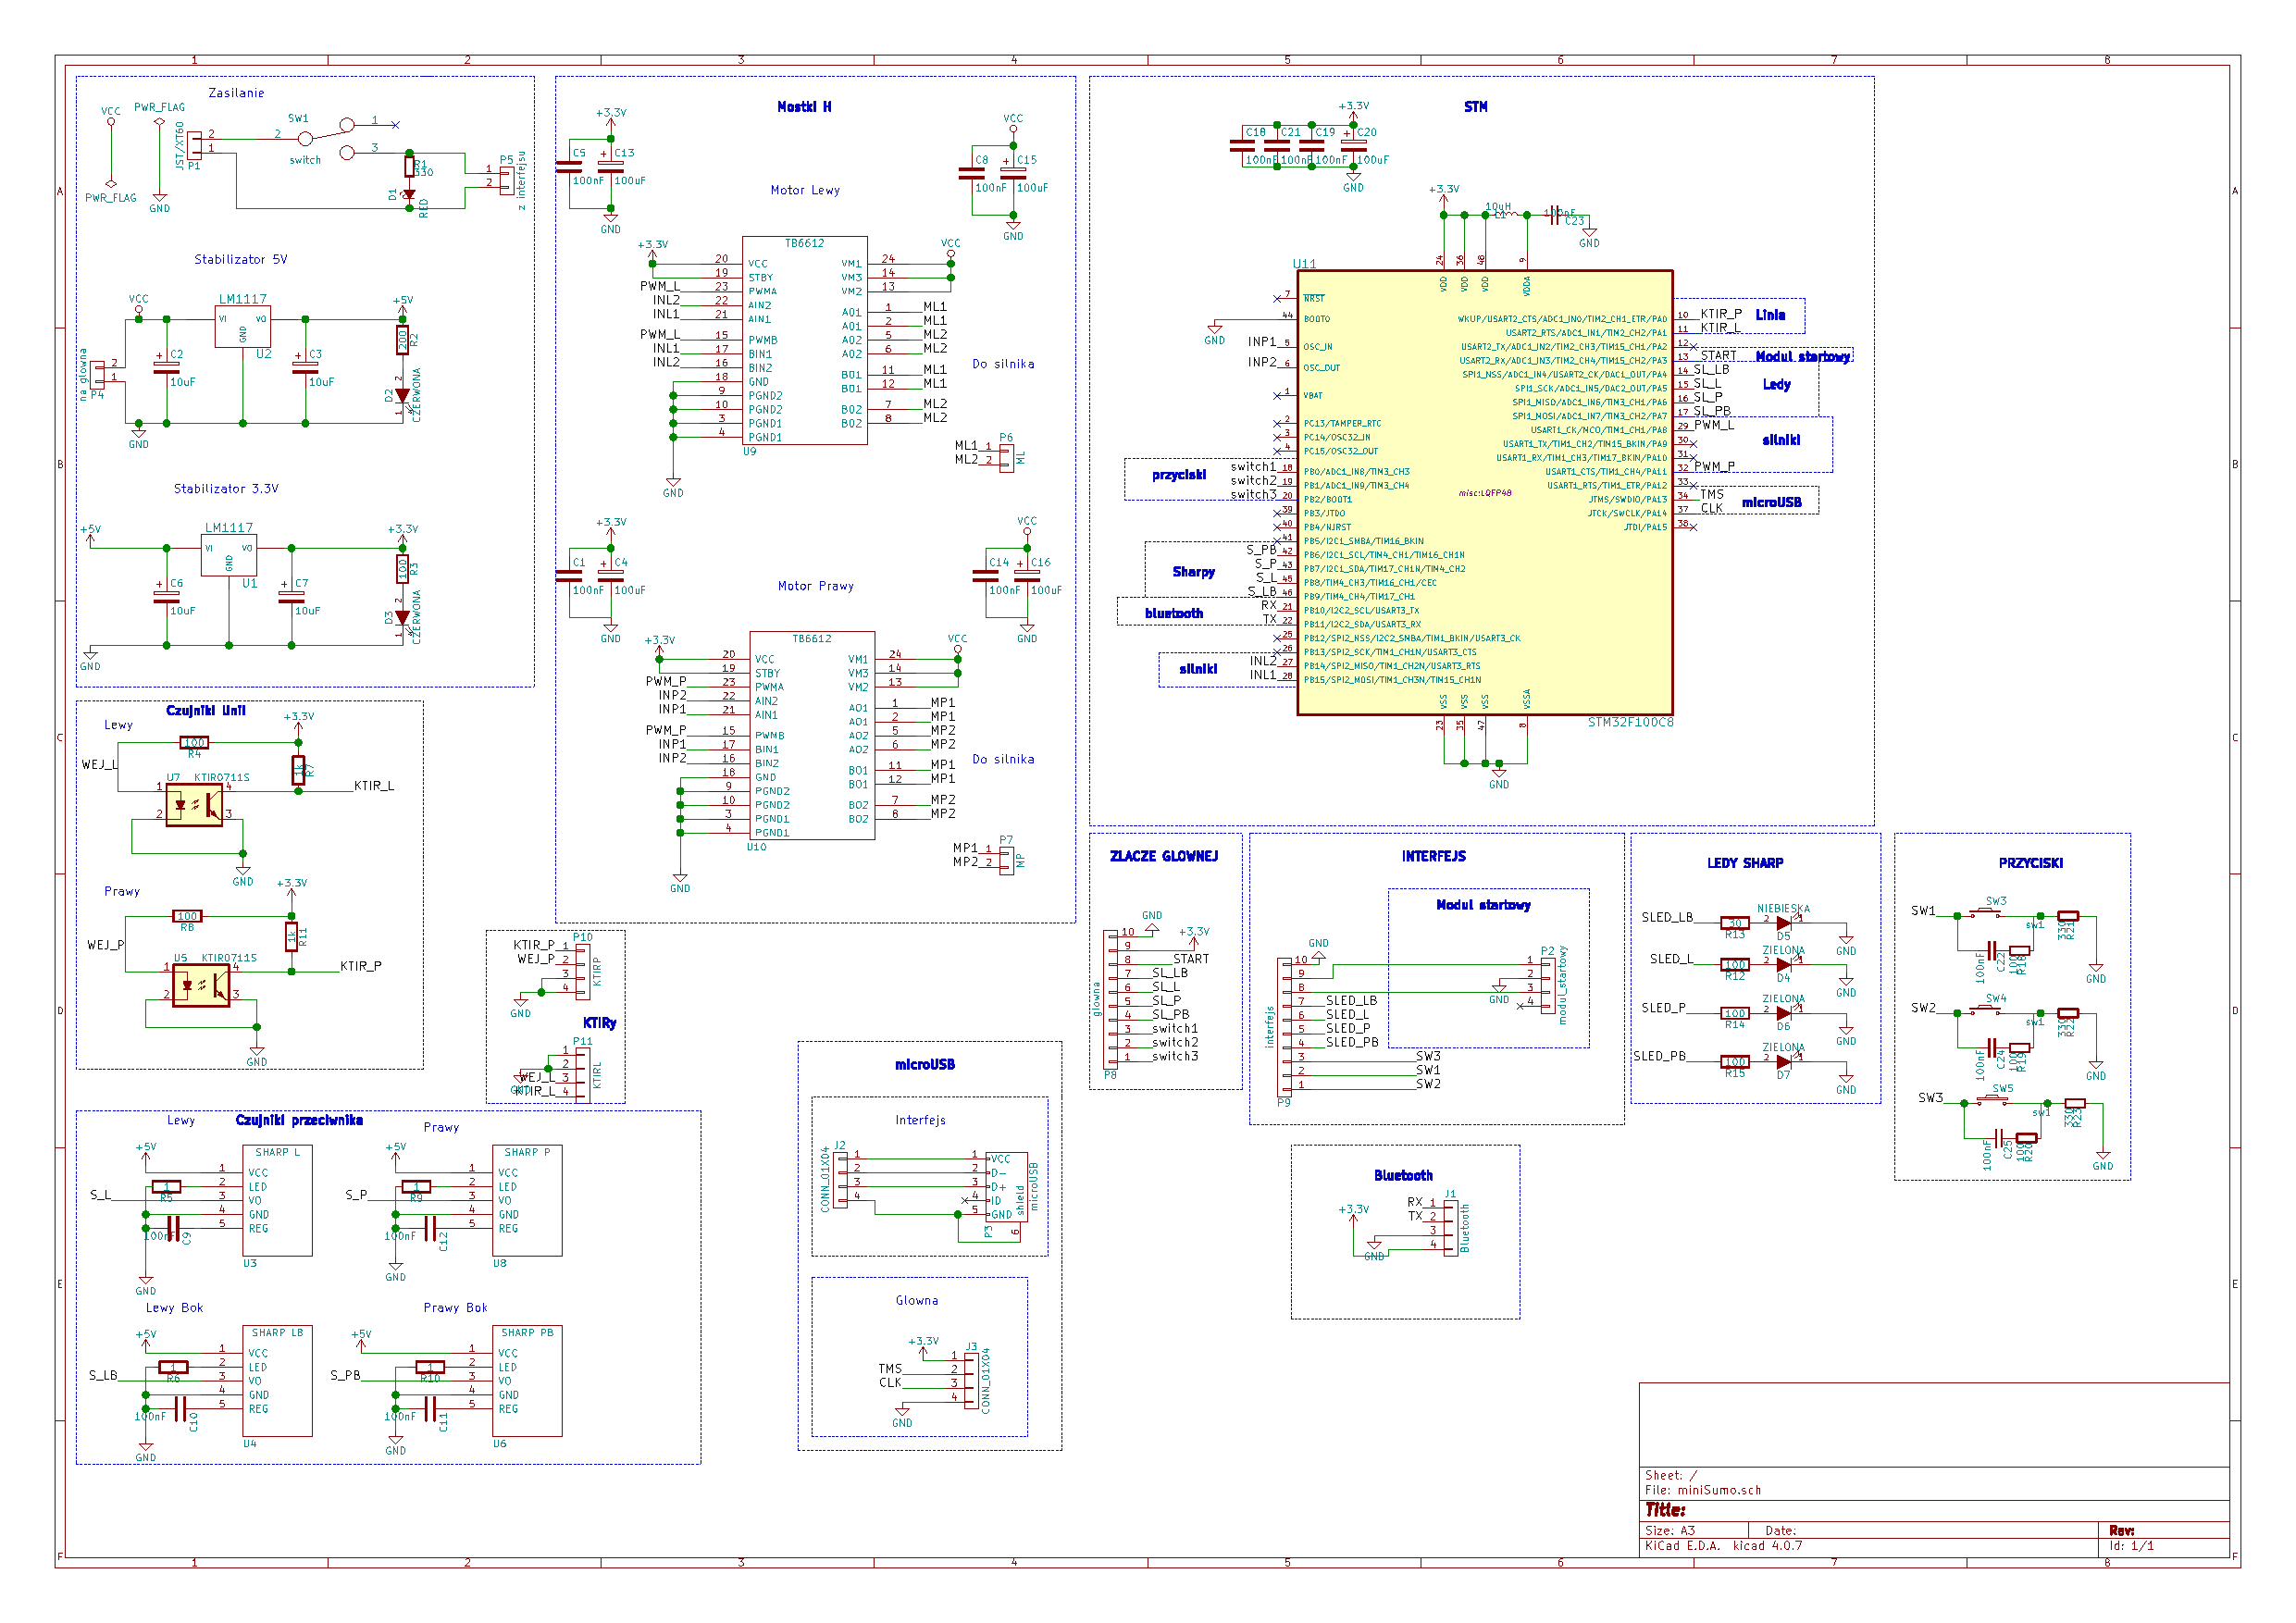
\includegraphics[width=0.8\linewidth]{pic04/electricscheme.pdf}
	\caption{Schemat elektroniki.}
	\label{fig:electric_scheme}	
\end{figure}
\end{landscape}

\section{Oprogramowanie}
Oprogramowanie sterujące robotem zostało napisane przy użyciu środowiska \textit{Eclipse}. Zawiera obsługę przychodzących/nadawanych wiadomości, zarządza sensoryką oraz motoryką konstrukcji. 

\subsection{Transmisja danych}
Transmisja danych opiera się na przesyłaniu ciągu liczb tak jak to opisano w 3 rozdziale. Przechwytywanie wiadomości odbywa się przy użyciu przerwania, które zostaje obsłużone w momencie zmiany stanu logicznego na pinie RX (połączonego z modułem Bluetooth) procesora. Następnie zostaje wywołana funkcja obsługująca przerwanie, przerywając tym samym aktualnie wykonywany kod. 

Listing \ref{interruptcode} przedstawia funkcję wywoływaną w momencie przerwania. Pierwszą czynnością było zapisanie odebranej wiadomości do zmiennej tablicowej \textit{received\_message},  Linia 6 przedstawia przypisanie pierwszej liczby otrzymanej wiadomości do zmiennej \textit{option} , która kolejno wykorzystywana jest w warunku \textit{switch} i w zależności od jej wartości ustawiane są odpowiednie flagi, będące zmiennymi globalnymi. Po zakończeniu działania opisywanej funkcji, program zostaje wznowiony w miejscu w którym został przerwany. 

Działanie głównej funkcji programu \textit{main()} wykorzystuje pętle, które przy każdej iteracji sprawdzają stan wyżej wspomnianych flag. Na ich podstawie określana jest obecnie wykonywana funkcjonalność robota. Reszta wiadomości parsowana jest przy użyciu metody \textit{parseValueFromMessage}, a następnie interpretowana w odpowiedni sposób, zależny od obecnie wykonywanej funkcjonalności.

\begin{minipage}{\textwidth}
	\begin{lstlisting}[label=interruptcode,caption=Funkcja obsługująca przerwanie.]
void HAL_UART_RxCpltCallback(UART_HandleTypeDef *huart) {

	sscanf((char*)receive_buffer, "%s", received_message);
	HAL_GPIO_TogglePin(GPIOA, led_bt_Pin);
	char option[1];
	option[0] = received_message[0];

	switch(atoi(option)) {
	case 1:
		automatic = true;
		HAL_UART_Receive_IT(&huart3, receive_buffer, 10);
		break;
	case 2:
		debug_motors = true;
		break;
	case 3:
		debug_tires = true;
		HAL_UART_Receive_IT(&huart3, receive_buffer, 10);
		break;
	case 4:
		debug_sensors = true;
		break;
	case 5:
		remote_joystick = true;
		break;
	case 6:
		remote_gyro = true;
		break;
	default:
		debug_tires = false;
		automatic = false;
		TIM1->CCR1 = 0;
		TIM1->CCR4 = 0;
		HAL_UART_Receive_IT(&huart3, receive_buffer, 10);
	    break;
	}
}
	\end{lstlisting}
\end{minipage}
 
\subsection{Sterowanie silnikami}
Sterowanie mocą silników odbywa się za pomocą modyfikacji wypełnienia sygnału przesyłanego do sterowników silników. Zakres wartości mieści się w przedziale 0 – 100 i określa procentowy czas trwania stanu wysokiego impulsu w pojedyncznym cyklu generowanym przez \textit{timer}. 

Poniższy listing \ref{pwmcode} przedstawia fragment kodu, który modyfikuje moc silników. \textit{TIM1} oznacza \textit{timer} generujący impuls, a \textit{CCR1} oraz \textit{CCR4} określają kanały, czyli docelowo silniki do których zostanie przesłany impuls.  Wartość wypełnienia zwracana jest przez metodę \textit{parseValueFromMessage}, która parsuje odpowiedni fragment wiadomości nadesłanej z aplikacji mobilnej. 

\begin{minipage}{\textwidth}
	\begin{lstlisting}[label=pwmcode,caption=Sterowanie mocą silników.]
TIM1->CCR1 = parseValueFromMessage(3,4);
TIM1->CCR4 = parseValueFromMessage(5,6);
	\end{lstlisting}
\end{minipage}

\subsection{Obsługa czujników}
Obsługa stanu czujników została zrealizowana w bardzo prosty sposób wynikający z charakterystyki pracy sensorów. W przypadku czujników wykrywających przeciwnika sprawdzany jest stan pinu procesora do którego podłączono wyjście sensoru. Sam czujnik działa na zasadzie diody podczerwonej generującej sygnał, który zostaje odbity od przeciwnika i trafia do odbiornika. Następnie na wyjściu czujnika występuje stan wysoki (logiczna 1) w przypadku braku przeciwnika lub stan niski (logiczne 0), gdy wykryto przeciwnika.

\begin{minipage}{\textwidth}
	\begin{lstlisting}[label=sharpcode,caption=Obsługa czujników przeciwnika.]
if(!HAL_GPIO_ReadPin(GPIOB, sharp_l_Pin))
	transmit_message[0] = 1;

if(!HAL_GPIO_ReadPin(GPIOB, sharp_ul_Pin))
	transmit_message[1] = 1;

if(!HAL_GPIO_ReadPin(GPIOB, sharp_ur_Pin))
	transmit_message[2] = 1;

if(!HAL_GPIO_ReadPin(GPIOB, sharp_r_Pin))
	transmit_message[3] = 1;
	\end{lstlisting}
\end{minipage}

Listing \ref{sharpcode} przedstawia kod, który sprawdza stan wyjścia czujników, a następnie w przypadku wykrycia przeciwnika zmienia wartość odpowiednych pól wiadomości, która zostanie przesłana do aplikacji mobilnej. 